% Gemini theme
% https://github.com/anishathalye/gemini

\documentclass[final]{beamer}

% ====================
% Packages
% ====================

\usepackage[T1]{fontenc}
\usepackage{lmodern}
\usepackage[size=custom,width=121.92,height=91.44,scale=1.3]{beamerposter}
\usetheme{gemini}
\usecolortheme{gemini}
\usepackage{graphicx}
\usepackage{booktabs}
\usepackage{tikz}
\usepackage{caption}
\usepackage{pgfplots}
\pgfplotsset{compat=1.14}
\usepackage{anyfontsize}

% ====================
% Lengths
% ====================

\newlength{\sepwidth}
\newlength{\colwidth}
\setlength{\sepwidth}{0.025\paperwidth}
\setlength{\colwidth}{0.3\paperwidth}

\newcommand{\separatorcolumn}{\begin{column}{\sepwidth}\end{column}}

% ====================
% Title
% ====================

\title{Power Play, Shot Selection, and \\ Scoring Outcomes in Elite Mixed Doubles Curling}
\author{Mark Zhang, University of Connecticut}

% ====================
% Body
% ====================

\begin{document}

\begin{frame}[t]
  \begin{columns}[t]

    \separatorcolumn
    % ==================== Column 1 ====================
    \begin{column}\colwidth
      \begin{block}{Abstract}

        The Power Play in mixed doubles curling allows the hammer team to reposition
        pre-placed stones to create a more aggressive setup, often aiming for multiple
        points. Despite its strategic importance, evidence on its effect on shot
        selection and end outcomes is limited. Using end-level data from the World
        Mixed Doubles Championships (2016–2025) and Olympic Winter Games (2018, 2022),
        we analyze how Power Play affects hammer-team shot selection and scoring. End
        outcomes are classified as 0, 1, or 2+ points, and shot selection is measured
        as the share of setup shots per end. We examine associations across score
        states and end timing, using a multinomial logit model adjusted for score
        state, end group, and team strength, supplemented by descriptive comparisons.
        Power Play is associated with more offensive shots, lower probability of zero
        points, higher probability of 2+ points, and increased expected scoring,
        especially in late-end comeback situations.
      \end{block}
      \begin{block}{Introduction}
        \begin{itemize}
          \item Mixed Doubles matches consist of 8 ends; each end begins with two stones
                pre-placed on the center line.
          \item The hammer team may exercise a one-time Power Play to shift these stones to the
                wings.
          \item Teams utilize the Power Play both offensively to generate multiple points and
                defensively to protect a lead.
        \end{itemize}
        \textbf{Research Questions}
        \begin{itemize}
          \item How does Power Play use affect hammer-team shot selection?
          \item How does Power Play influence end scoring outcomes?
          \item Which match contexts maximize Power Play effectiveness?

        \end{itemize}
      \end{block}
      \begin{block}{Data}
        \begin{itemize}
          \item Shot-level data from World Championships and Olympics is aggregated to end
                level. \cite{ritchie2025opening}
          \item Score state is calculated from the hammer team’s perspective.
          \item Outcome: points scored (0 / 1 / 2+); shot selection: share of offensive/setup
                shots
        \end{itemize}

        \begin{center}
          \textbf{Key Variables}
        \end{center}

        \centering
        \begin{tabular}{lll}
          \toprule
          Variable       & Symbol    & Description                           \\
          \midrule
          Power Play     & $x_{PP}$  & 1 = used, 0 = not used                \\
          Score state    & $x_S$     & Leading / Tied / Trailing             \\
          End group      & $x_E$     & Early ($\le 6$) / Late ($\ge 7$)      \\
          Outcome        & $Y$       & Points scored: 0 / 1 / 2+             \\
          Strength diff  & $x_{str}$ & Standardized team strength difference \\
          Offensive Rate & $p$       & Draw, Guard, Freeze shots / Total     \\
          \bottomrule
        \end{tabular}
      \end{block}

    \end{column}

    \separatorcolumn
    % ==================== Column 2 ====================
    \begin{column}\colwidth
      \begin{block}{Descriptive Statistics}

        \centering
        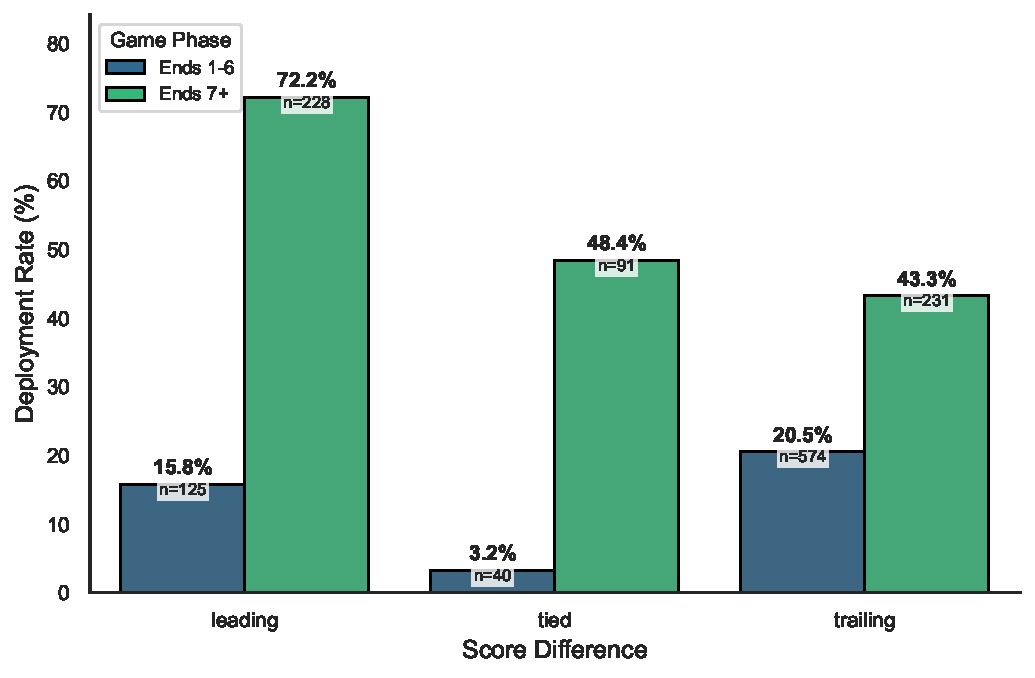
\includegraphics[width=.9\linewidth]{../manuscript/figures/usage.pdf}
        \\
        {\small Power Play deployment frequency by game phase and score.}
        \begin{itemize}
          \item Hammer teams are disproportionately in trailing score states.
          \item Power Play deployment peaks in late ends when leading.
        \end{itemize}
      \end{block}

      \begin{block}{Methods}
        We analyzed the \textbf{Power Play (PP)} using two models with
        cluster-robust standard errors by unique match. Let $\mathbf{x}$ represent
        the design vector and $\boldsymbol{\beta}$ the coefficient vector:

        \[ \mathbf{x} = [1, x_{PP}, x_S, x_E, x_{PP}x_S, x_{PP}x_E, x_{str}]^\top. \]
        \[ \boldsymbol{\beta} = [\beta_0, \beta_1, \beta_2, \beta_3, \beta_4, \beta_5, \beta_6]^\top. \]

        \textbf{1. Shot Selection (Binomial GLM)}: \\
        The probability $p$ of an offensive shot is modeled as:
        \[ \text{logit}(p) = \mathbf{x}^\top \boldsymbol{\beta}. \]

        \textbf{2. Scoring Outcomes (Multinomial Logit)}: \\
        For outcomes $j \in \{1, 2+\}$ relative to a 0-point baseline, the log-odds are:
        \[ \ln\left(\frac{\Pr(Y=j)}{\Pr(Y=0)}\right) = \mathbf{x}^\top \boldsymbol{\beta}_j. \]
      \end{block}

      \begin{block}{Results: Predicted Shot Selection}

        \centering
        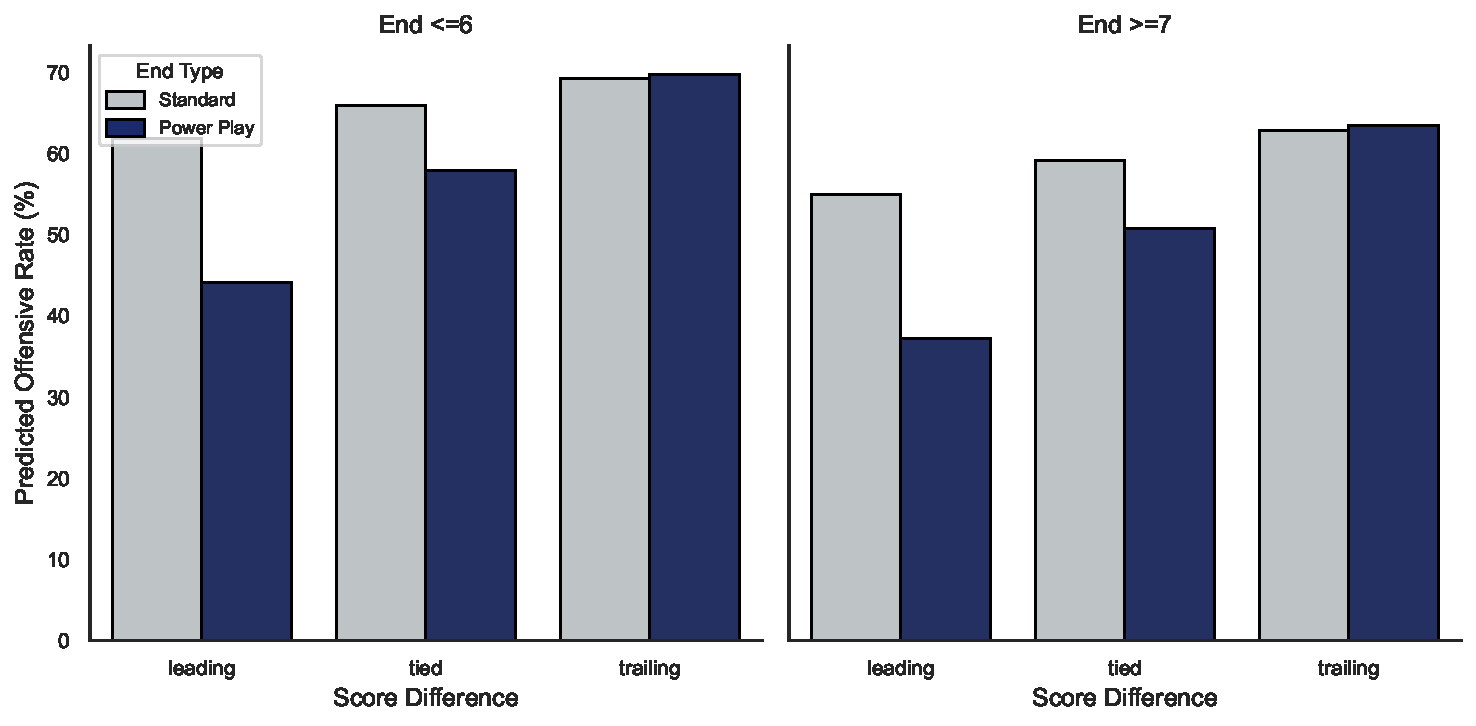
\includegraphics[width=.9\linewidth]{../manuscript/figures/strategy.pdf}
        \\
        {\small Predicted hammer offensive shot rates (\%) from Binomial GLM.}
        \begin{itemize}
          \item Leading teams play a lower proportion of offensive shots.
          \item Hammer teams typically play more offensively in standard ends, except for when
                trailing in early ends.
        \end{itemize}
      \end{block}

    \end{column}
    \separatorcolumn
    % ==================== Column 3 ====================
    \begin{column}\colwidth
      \begin{block}{Results: Predicted Scoring Outcomes}
        \centering

        % --- Table Section ---
        \begin{table}
          \caption*{\textbf{Scoring Dynamics: Relative Risk Ratios [95\% CI]}}
          \begin{tabular}{lll}
            \toprule
            Predictor                & Prob (1 Pt)          & Prob (2+ Pts)        \\
            \midrule
            Score: Leading           & 1.12 [0.90, 1.38]    & 1.28** [1.04, 1.57]  \\
            Score: Tied              & 1.15 [0.97, 1.36]    & 1.06 [0.89, 1.27]    \\
            End $\geq$ 7 (Late)      & 0.82* [0.65, 1.03]   & 0.76** [0.60, 0.96]  \\
            Power Play (PP)          & 1.66*** [1.33, 2.09] & 2.57*** [2.06, 3.21] \\
            PP $\times$ Leading      & 0.87 [0.57, 1.33]    & 0.54*** [0.36, 0.83] \\
            PP $\times$ Tied         & 0.52** [0.30, 0.90]  & 0.57** [0.33, 0.97]  \\
            PP $\times$ End $\geq$ 7 & 1.21 [0.82, 1.79]    & 1.42* [0.97, 2.09]   \\
            Team Strength (Z)        & 1.26*** [1.17, 1.35] & 1.87*** [1.74, 2.01] \\
            \bottomrule
          \end{tabular}

          \smallskip

          {\small \textit{Note:} RRR relative to 0-point outcome. Baseline: Trailing, Ends 1--6.\\
            Significance: * $p<0.05$, ** $p<0.01$, *** $p<0.001$. $N=5861$ ends.}
        \end{table}
        \begin{itemize}
          \item Power Play usage is associated with significantly higher odds of both 1 and 2+
                point scoring outcomes.
          \item The marginal benefit of the Power Play diminishes for teams that are tied or
                leading.
          \item Higher team strength (Z-score) consistently increases scoring odds.
        \end{itemize}
        \vspace{0.5em}
        % --- Figure Section ---
        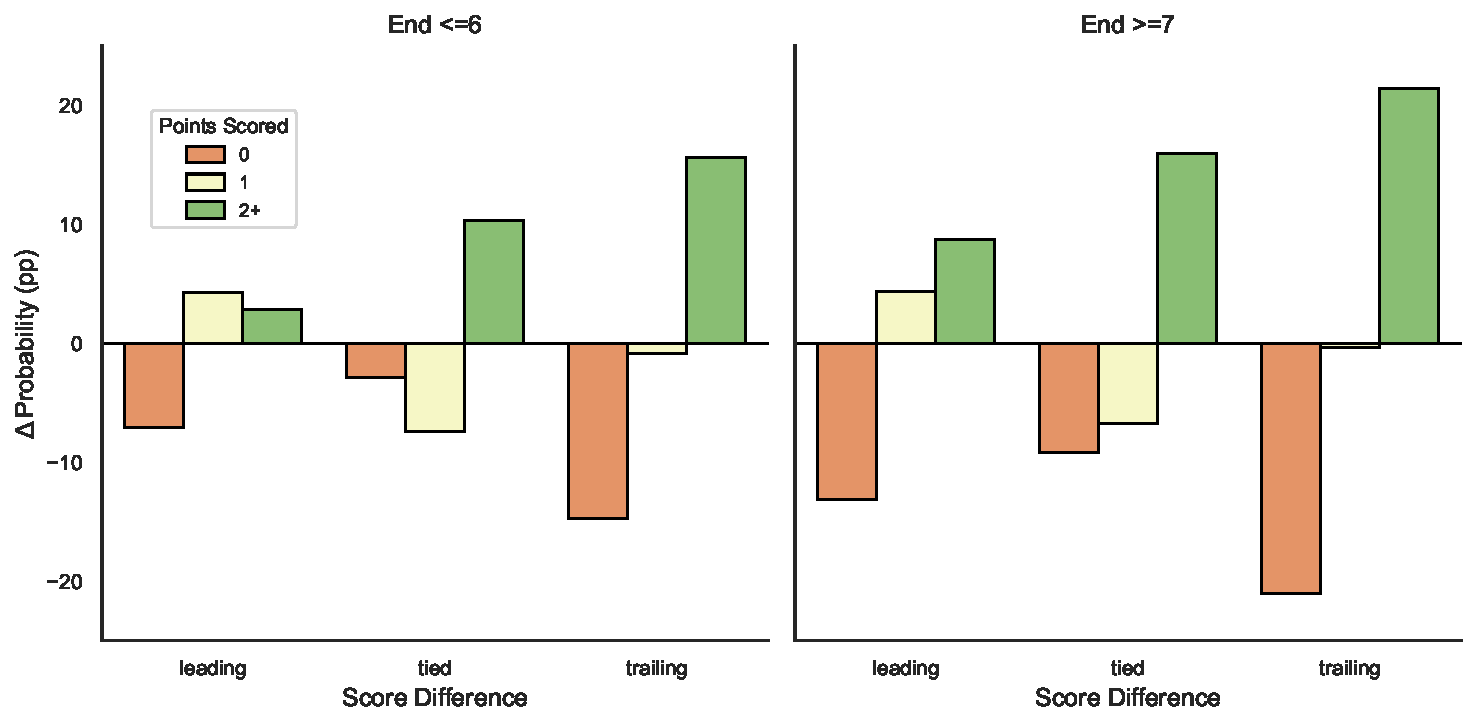
\includegraphics[width=.95\linewidth]{../manuscript/figures/outcomes.pdf}

        {\small Predicted hammer score probabilities of 2+ points from Multinomial Logit.}

        \vspace{0.5em}

        \begin{itemize}
          \item Late ends show a lower probability of scoring 2+ points in standard play, but a
                substantial increase under Power Play.
          \item Trailing teams in late ends exhibit the highest model-predicted probability of
                scoring 2+ points via the Power Play.
        \end{itemize}
      \end{block}
      \begin{alertblock}{Discussion}
        \begin{itemize}
          \item Power Play usage is associated with a significantly higher probability of
                scoring 2+ points for trailing teams.
          \item Conversely, leading teams deploy the Power Play to simplify the house and
                minimize steal risks.
          \item These findings suggest that elite teams calibrate shot selection and tactical
                risk based on match context.

        \end{itemize}

      \end{alertblock}

      \heading{References}
      \nocite{*}
      {\small
        \bibliographystyle{plain}
        \bibliography{poster}
      }

    \end{column}
    \separatorcolumn
  \end{columns}
\end{frame}
\end{document}